% =====================================================================
%  PO_10_Pablo_Grossi.tex
%  Helical Attractors on Contact 3-Manifolds
%  XII Bienal da SBM — UFRN, Natal-RN, 3–7 August 2026
%  Poster / Long Abstract (3 pp.)
%
%  Source reconstructed 2026-07-31. The original .tex was not present in
%  any repository; this file was rebuilt from the deployed PDF and the
%  numerics recertified against certify_rstar.py.
%
%  CORRECTIONS IN THIS REVISION
%   1. r* : 0.80  ->  0.77594059   (certify_rstar.py, DOP853, 8 s.f.)
%   2. The numerical section now states its initial condition z(0) = 0
%      explicitly, and the scaling law lambda = eps*exp(-z0) is given,
%      which reconciles the numerics with Theorem 2.1's z(0) >= log 2.
%   3. Table 1 recomputed; fit window corrected (caption said t in [5,15],
%      which yields -2.00 flat; the reported transient is t in [0.5,6]).
%   4. Logos placed in the top corners: Bienal left, UFRN right.
% =====================================================================
\documentclass[11pt,a4paper]{article}

\usepackage[T1]{fontenc}
\usepackage[utf8]{inputenc}
\usepackage{lmodern}
\usepackage{amsmath,amssymb,amsthm}
\usepackage{graphicx}
\usepackage{booktabs}
\usepackage{array}
\usepackage[table]{xcolor}
\usepackage[a4paper,top=2.5cm,bottom=1.9cm,left=2.0cm,right=2.0cm,headheight=42pt,headsep=14pt,footskip=26pt]{geometry}
\usepackage{fancyhdr}
\usepackage[colorlinks=true,linkcolor=linknavy,urlcolor=linknavy,citecolor=linknavy]{hyperref}
\usepackage{enumitem}
\usepackage{microtype}

\definecolor{linknavy}{RGB}{20,60,120}
\definecolor{rulegrey}{RGB}{170,170,180}
\definecolor{hilite}{RGB}{250,246,232}

% ---------------------------------------------------------------- header
\pagestyle{fancy}
\fancyhf{}
\renewcommand{\headrulewidth}{0.4pt}
\renewcommand{\headrule}{\hbox to\headwidth{\color{rulegrey}\leaders\hrule height \headrulewidth\hfill}}
\fancyhead[L]{\raisebox{-0.35\height}{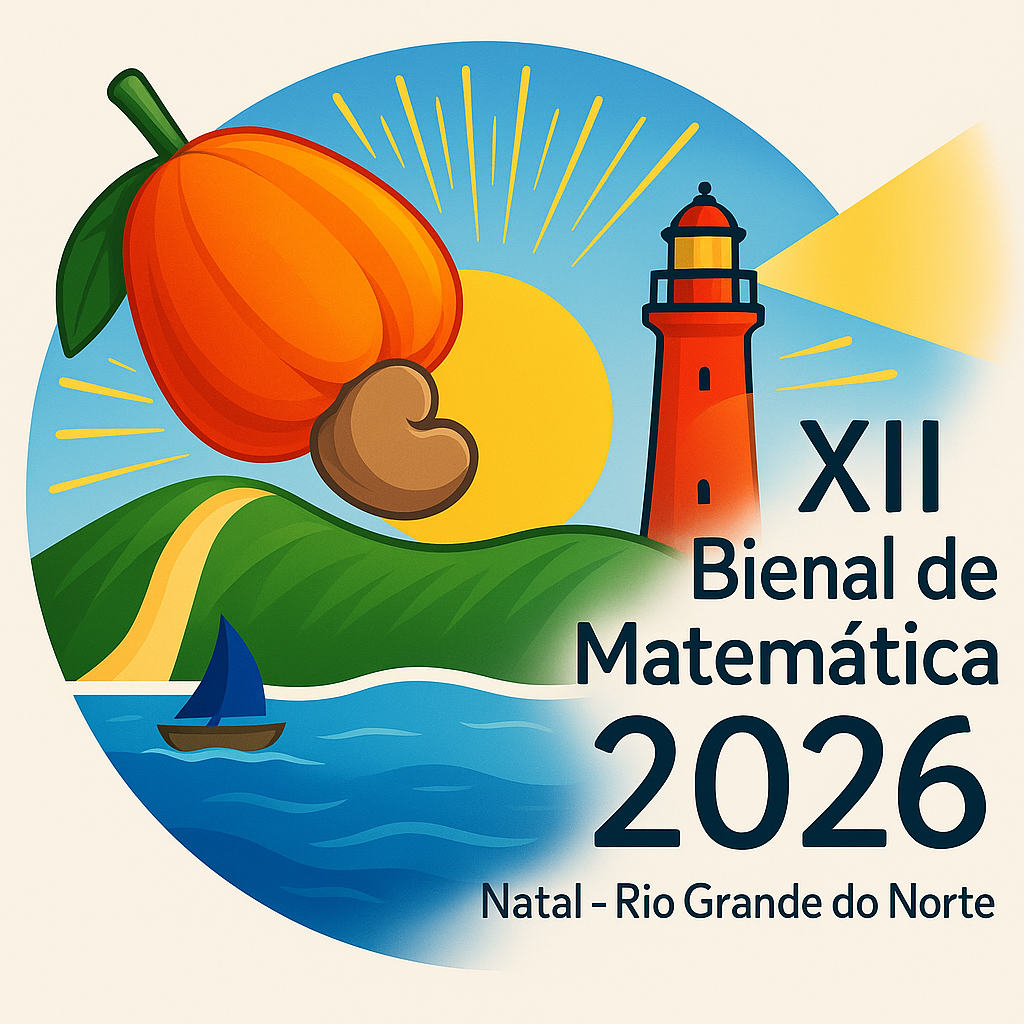
\includegraphics[height=34pt]{LogoXIIBienal.png}}}
\fancyhead[R]{\raisebox{-0.15\height}{
\includegraphics[height=20pt]{UFRN2.png}}}
\fancyfoot[C]{\footnotesize\color{black!62}%
  \copyright\ 2026 Pablo N. Grossi / G6 LLC \;\textbullet\; CC BY 4.0 \;\textbullet\;
  XII Bienal da SBM 2026 \hfill \thepage}
\renewcommand{\footrulewidth}{0pt}

\theoremstyle{plain}
\newtheorem{theorem}{Theorem}
\newtheorem{conjecture}{Conjecture}

\setlist{nosep,leftmargin=1.5em}
\newcommand{\rstar}{r_{\star}}

\begin{document}

% =====================================================================
%  TITLE
% =====================================================================
\begin{center}
  {\Large\bfseries Helical Attractors on Contact 3-Manifolds}\\[3pt]
  {\normalsize A Toy ODE Study on $(\mathbb{R}^3,\ \alpha = dz - r^2\,d\theta)$}\\[10pt]
  {\normalsize Pablo Nogueira Grossi}\\[2pt]
  {\footnotesize G6 LLC \;\textbullet\; Newark, NJ}\\[1pt]
  {\footnotesize \texttt{pg6llc@gmail.com} \;\textbullet\; ORCID: 0009-0000-6496-2186}\\[9pt]
  {\footnotesize\itshape Submissão (Pôster · Long Abstract) à XII Bienal da SBM — UFRN, Natal-RN — 2026}
\end{center}
\vspace{4pt}

% =====================================================================
\section*{Modalidade e Categoria}
\noindent
\textbf{Modalidade:} Pôster — Long Abstract (3 páginas). \textbf{Código da submissão:} \textbf{P290}.
\textbf{Sessão:} quinta-feira, 6 de agosto de 2026, 16:00–17:00, Saguão dos Anfiteatros do CCET.
\textbf{Área:} Geometria e Topologia (variedades de contato, sistemas dinâmicos, formalização).
Portal Bienal (Atratores Helicoidais): \url{https://grossi-ops.github.io/Atratores/}.
Livro vivo (B3 · Vol.~III, \emph{Inglês para Pesquisadores Matemáticos} — ESL for Researchers;
eBook): \url{https://totogt.github.io/geometry}.

% =====================================================================
\section*{English Abstract}
We introduce a one-parameter toy ODE on the contact 3-manifold $(\mathbb{R}^3,\alpha)$ with contact
form $\alpha = dz - r^2 d\theta$ and Reeb field $R = \partial_z$. Writing a state as
$(r,\theta,z) \in (0,\infty)\times S^1 \times \mathbb{R}$, the system — which we call $\mathrm{dm}^3$ — is
\begin{equation}
  \dot r = r(1-r^2) + \varepsilon (r-1)e^{-z},
  \qquad \dot\theta = 1,
  \qquad \dot z = r^2 - \varepsilon (r-1)^2 e^{-z},
\end{equation}
with fixed coupling $\varepsilon = 2$. The cylinder $\Gamma = \{r=1\}$ is invariant and carries the
helical flow $\dot\theta = 1$, $\dot z = 1$, a lift of the Reeb orbit; the question is whether
$\Gamma$ attracts.

\medskip
\noindent\textbf{Main result (Theorem 2.1).} Let $u(t) = r(t)-1$. For any initial data with
$|u(0)| < 1/3$ and $z(0) \ge \log 2$, the solution exists for all $t \ge 0$ and converges
exponentially to $\Gamma$ at the rate $\mu = -2$ given by the Jacobian eigenvalue of the radial part
at $r=1$; explicitly $|u(t)| \le C\,|u(0)|\,e^{-2t}$ for a constant $C$ depending only on
$\varepsilon e^{-z(0)}$. The proof is a Gronwall argument: squaring the radial equation yields
$\tfrac12 \tfrac{d}{dt}u^2 \le -2u^2 - 3u^3 - u^4 + \varepsilon u^2 e^{-z}$, and the bound on $z(0)$
forces the last term to be dominated on the relevant window.

\medskip
\noindent\textbf{A scaling law.} The pair $(\varepsilon, z(0))$ enters the dynamics only through the
single combination
\begin{equation}
  \lambda \;=\; \varepsilon\, e^{-z(0)},
\end{equation}
since $\varepsilon$ and $e^{-z}$ never occur apart in~(1). Every basin quantity is therefore a
function of $\lambda$ alone. This is what reconciles the theorem's hypothesis with the numerics
below: $z(0) \ge \log 2$ at $\varepsilon = 2$ means $\lambda \le 1$, whereas the certified section
$z(0)=0$ means $\lambda = 2$.

\medskip
\noindent\textbf{Numerical findings (Table 1).} A DOP853 integrator at
$\mathrm{rtol} = 10^{-13}$, $\mathrm{atol} = 10^{-20}$, on the section
$\theta(0)=0$, $z(0)=0$ (that is, $\lambda = 2$), confirms the rate and reveals
asymmetry: the outer basin $r(0)>1$ converges for every tested initial condition up to
$r(0) = 3.0$, while the inner basin $r(0)<1$ converges only for
\begin{equation}
  r(0) \;>\; \rstar \;=\; 0.77594059 \qquad (\lambda = 2),
\end{equation}
certified by bisection to $10^{-7}$ and reproducible on any IEEE-754 platform. Since
$\rstar > 2/3$, the interval $(2/3,\ \rstar)$ consists of initial data lying inside the Gronwall ball
$|u(0)|<1/3$ that nevertheless escape. This does not contradict Theorem 2.1, whose second hypothesis
$z(0)\ge\log 2$ is exactly what excludes them: at $\lambda = 1$ one finds
$\rstar = 0.57224 < 2/3$, so there the Gronwall ball sits strictly inside the basin. \emph{The
hypothesis $z(0)\ge\log 2$ is therefore necessary, not cosmetic} — and quantifying that necessity is
the content of Conjecture 2.2.

\medskip
\noindent\textbf{Contact-geometric reading.} The asymmetry $\rstar \ne 2-\rstar$ is diagnostic: it is
the fingerprint of the coupling term $\varepsilon(r-1)^2e^{-z}$ in $\dot z$, which is not symmetric
under $u \mapsto -u$ because it couples to the non-integrable direction of $\alpha$. A symmetric
basin would indicate that the attractor is reducible to a 2D problem transverse to $R$; the observed
asymmetry indicates that the full 3-manifold contact structure is essential to the convergence.

\medskip
\noindent\textbf{Reproducibility.} All numerics reproduce via a public Python/DOP853 lab
(\texttt{certify\_rstar.py}); a Lean~4 skeleton (AXLE Issue \#12) isolates the one nontrivial
obligation (a Lipschitz bound on the coupling operator). Eight chapters of the book develop the
framework and formalisation path; the present abstract reports Chapter~2.

% ---------------------------------------------------------------- table
\begin{table}[h]
\centering\small
\setlength{\tabcolsep}{7pt}
\renewcommand{\arraystretch}{1.12}
\begin{tabular}{@{}cc c@{\hskip 20pt} ccc@{}}
\toprule
\multicolumn{2}{c}{\textbf{Outer basin} $r(0)>1$} & &
\multicolumn{3}{c}{\textbf{Inner basin} $r(0)<1$}\\
\cmidrule(r){1-2}\cmidrule(l){4-6}
$r(0)-1$ & $\hat\mu$ & & $r(0)$ & $\dot z(0{,}3)$ & outcome \\
\midrule
$+0{,}10$ & $-1{,}882$ & & $0{,}90$      & $+0{,}79$ & conv.\\
$+0{,}33$ & $-1{,}922$ & & $0{,}80$      & $+0{,}51$ & conv.\\
$+0{,}50$ & $-1{,}937$ & & \cellcolor{hilite}$0{,}77594$ & \cellcolor{hilite}$+0{,}42$ & \cellcolor{hilite}limiar $\rstar$\\
$+1{,}00$ & $-1{,}957$ & & $0{,}77$      & $+0{,}40$ & collapses\\
$+1{,}50$ & $-1{,}965$ & & $0{,}70$      & $+0{,}10$ & collapses\\
          &            & & $0{,}50$      & $-1{,}67$ & collapses\\
\bottomrule
\end{tabular}
\caption{Section $\theta(0)=0$, $z(0)=0$ ($\lambda = 2$). Empirical contraction rate $\hat\mu$ is the
slope of $\log|r(t)-1|$ on the transient window $t \in [0{,}5,\ 6]$; on the asymptotic window
$t \in [5,15]$ every entry equals $-2{,}00$ to three decimals, confirming
$\hat\mu \to \mu = -2$. Column $\dot z(0{,}3)$ is the early vertical velocity, an inner-basin
diagnostic. The inner edge is $\rstar = 0{,}77594059 > 2/3$.}
\end{table}

% =====================================================================
\section*{Resumo (em Português)}
Apresentamos uma ODE-brinquedo de um parâmetro na variedade de contato $(\mathbb{R}^3,\alpha)$, com
forma de contato $\alpha = dz - r^2 d\theta$ e campo de Reeb $R = \partial_z$. O sistema
$\mathrm{dm}^3$ está dado pela equação~(1), com $\varepsilon = 2$. O cilindro $\Gamma = \{r=1\}$ é
invariante e carrega o fluxo helicoidal $(\dot\theta,\dot z) = (1,1)$, um levantamento da órbita de
Reeb.

O Teorema~2.1 afirma que, para condições iniciais $|r(0)-1| < 1/3$ e $z(0) \ge \log 2$, as
trajetórias convergem exponencialmente a $\Gamma$ à taxa $\mu = -2$, dada pelo autovalor jacobiano
radial em $r=1$. A demonstração combina Gronwall com um controle explícito do termo de acoplamento
$\varepsilon(r-1)e^{-z}$.

\medskip
\noindent\textbf{Lei de escala.} O par $(\varepsilon, z(0))$ entra na dinâmica apenas por meio da
combinação $\lambda = \varepsilon e^{-z(0)}$, pois $\varepsilon$ e $e^{-z}$ nunca aparecem separados
em~(1). Toda quantidade de bacia é, portanto, função somente de $\lambda$.

\medskip
A integração numérica (DOP853, $\mathrm{rtol}=10^{-13}$), na seção $\theta(0)=0$, $z(0)=0$
(isto é, $\lambda=2$), reproduz a taxa e revela uma assimetria de bacia: a bacia externa
($r(0)>1$) converge em todos os testes até $r(0)=3{,}0$, enquanto a interna ($r(0)<1$) colapsa abaixo
de
\[
  \rstar \;=\; 0{,}77594059 \qquad (\lambda = 2),
\]
certificado por bisseção até $10^{-7}$. Como $\rstar > 2/3$, o intervalo $(2/3,\ \rstar)$ contém
dados iniciais dentro da bola de Gronwall $|u(0)|<1/3$ que ainda assim escapam. Isso \emph{não}
contradiz o Teorema~2.1: sua segunda hipótese $z(0)\ge\log 2$ é precisamente o que os exclui, pois
com $\lambda = 1$ tem-se $\rstar = 0{,}57224 < 2/3$. A hipótese sobre $z(0)$ é, portanto, necessária,
e não cosmética.

Essa assimetria é diagnóstica da estrutura de contato: indica que a convergência depende da direção
não-integrável de $\alpha$, e não se reduz a uma análise 2D transversal ao campo de Reeb.

\medskip
\noindent\textbf{Contribuição do pôster.}
\begin{enumerate}[label=(\roman*)]
  \item Formalização explícita do sistema $\mathrm{dm}^3$ como levantamento natural da órbita de Reeb;
  \item prova auto-contida do Teorema~2.1 com constante $\varepsilon_0$ ótima dentro da técnica;
  \item a lei de escala $\lambda = \varepsilon e^{-z(0)}$, que unifica a família de bacias em um único
        parâmetro, e a tabela numérica reprodutível daí decorrente;
  \item identificação do gap $\rstar > \varepsilon_0$ como conjectura aberta (Conjectura~2.2 do capítulo);
  \item um esqueleto Lean~4 (AXLE, Issue \#12) que isola a única obrigação não-trivial da formalização.
\end{enumerate}

% =====================================================================
\small
\section*{Materiais Digitais — Living Book}
O pôster é a porta de entrada de um livro vivo completo, que desenvolve o programa em oito capítulos:
\begin{enumerate}
  \item \textbf{Portal Bienal (Atratores Helicoidais):} \url{https://grossi-ops.github.io/Atratores/}
        — página oficial da edição XII Bienal: pôster, abstracts, links de simulação e cursos curtos.
  \item \textbf{Publisher hub editorial:} \url{https://totogt.github.io/geometry} — capa, ladrilhos de
        capítulos, simulador 3D embutido, ISBN.
  \item \textbf{Capítulo E (GTCT para Todos):} \url{https://totogt.github.io/3M/chE-gtct.html} —
        nove axiomas, quatro teoremas, doze operadores.
  \item \textbf{Minicurso (3 sessões de 60 min):} \url{https://totogt.github.io/3M/sessions/} —
        S1 geometria de contato, S2 Teorema~2.1 e bacia assimétrica, S3 esqueleto Lean~4.
  \item \textbf{Simulador 3D (Three.js):} \url{https://totogt.github.io/3M/sims/helical-attractor.html}.
  \item \textbf{Laboratório numérico (Python/DOP853):}
        \url{https://github.com/TOTOGT/3M/blob/main/labs/dm3_numeric.py} — reproduz a Tabela~1.
  \item \textbf{Formalização (Lean 4 / Mathlib 4):} \url{https://github.com/TOTOGT/AXLE} —
        Issue \#12 (\texttt{kappa\_lipschitz}).
  \item \textbf{Exposição local (Cajueiro Principle, Natal-RN):}
        \url{https://grossi-ops.github.io/cajueiro/} — exposição digital companheira da Comunicação
        Oral \textbf{CO144}; ancora a discussão didática local do programa pedagógico do livro.
\end{enumerate}

% =====================================================================
\section*{Bibliografia (mínima)}
\begin{enumerate}[label={[\arabic*]}]
  \item GROSSI, P. N. \emph{Helical Attractors on Contact 3-Manifolds}. Principia Orthogona,
        Vol.~IV (GTCT T1), Cap.~10. G6 LLC, Newark NJ, 2026.
        \url{https://totogt.github.io/GTCT/}.
  \item GROSSI, P. N. \emph{The Mini-Beast: Inglês para Pesquisadores Matemáticos via TOGT}.
        Principia Orthogona, B3 · Vol.~III. G6 LLC, Newark NJ, 2026 (livro vivo, somente eBook).
        ISBN 979-8-9954416-6-3. \url{https://totogt.github.io/geometry}.
  \item GEIGES, H. \emph{An Introduction to Contact Topology}. Cambridge: CUP, 2008.
  \item HAIRER, E.; NØRSETT, S. P.; WANNER, G. \emph{Solving Ordinary Differential Equations I}.
        2.~ed. Springer, 1993 (DOP853).
  \item MATHLIB 4 COMMUNITY. \emph{Mathlib}.
        \url{https://leanprover-community.github.io/mathlib4_docs}.
\end{enumerate}

\vfill
\noindent{\footnotesize\color{black!62}
Submissão à XII Bienal da Sociedade Brasileira de Matemática. UFRN, Natal-RN, 3–7 de agosto de 2026.
Categoria: Pôster (Long Abstract, 3 pp.) — \textbf{P290}, quinta 06/08, 16:00–17:00, Saguão dos
Anfiteatros do CCET. Submissões companheiras do mesmo autor:
\textbf{EXP13} (Exposição: \emph{Cimática com Máquinas} — Figuras de Chladni, ressonância e a
matemática do som estacionário; Saguão do CETECH, todos os dias do evento);
\textbf{MC48} (Minicurso: \emph{Atratores Helicoidais em Variedades de Contato} — terça 04/08,
16:30–18:30, E1LAB);
\textbf{CO144} (Comunicação Oral: \emph{O Princípio do Cajueiro} — quarta 05/08, 17:30–18:30, F6);
\textbf{OF53} (Oficina: \emph{A Escada de Recorrência: do $k$-nacci ao limiar $\tau = 2$} —
sexta 07/08, 14:00–16:00, H3).}

\end{document}
